\documentclass[11pt,twoside,a4paper]{book}  
% definice dokumentu
\usepackage[czech, english]{babel}
\usepackage[T1]{fontenc} 				% pouzije EC fonty 
\usepackage[utf8]{inputenc} 			% utf8 kódování vstupu 
\usepackage[square, numbers]{natbib}	% sazba pouzite literatury
\usepackage{indentfirst} 				% 1. odstavec jako v~cestine, pro práci v~aj možno zakomentovat
\usepackage{fancyhdr}					% tisk hlaviček a~patiček stránek
\usepackage{nomencl} 					% umožňuje snadno definovat zkratky a~jejich seznam

%%%%%%%%%%%%%%%%%%%%%%%%%%%%%%%%%%%%%%%%%%%%%%%%%%%%%%%%%%%%%%%
% informace o práci
\newcommand\WorkTitle{Software pro distribuované řízení a vyčítání dat ze sítě částiových pixelových detektorů Timepix3} % název
\newcommand\FirstandFamilyName{Bc. Jakub Begera} % autor
\newcommand\Supervisor{Ing. Štěpán Polanský} % vedoucí

\newcommand\TypeOfWork{Diplomová práce}	% typ práce [Diplomová práce | Bakalářská práce | Bachelor's Project | Master's Thesis ]	

% Nastavte následují podle vašeho oboru a~programu (pomoc hledejte na http://www.fel.cvut.cz/cz/education/bk/prehled.html)								
\newcommand\StudProgram{Otevřená informatika} % program
\newcommand\StudBranch{Softwarové inženýrství} % obor

%%%%%%%%%%%%%%%%%%%%%%%%%%%%%%%%%%%%%%%%%%%%%%%%%%%%%%%%%%%%%%%
% minimální importy
\usepackage{graphicx}					% pro vkládání obrázků
\usepackage{k336_thesis_macros} 		% specialni makra pro formatovani DP a~BP
\usepackage[
pdftitle={\WorkTitle},				% nastaví v~informacích o pdf název
pdfauthor={\FirstandFamilyName},	% nastaví v~informacích o pdf autora
colorlinks=true,					% před tiskem doporučujeme nastavit na false, aby odkazy a~url nebyly šedé při ČB tisku
breaklinks=true,
urlcolor=red,
citecolor=blue,
linkcolor=blue,
unicode=true,
]
{hyperref}								% pro zobrazování "prokliknutelných" linků 

% rozšiřující importy
\usepackage{listings} 			%slouží pro tisk zdrojových kódů se syntax higlighting
\usepackage{algorithmicx} 		%slouží pro zápis algoritmů
\usepackage{algpseudocode} 		%slouží pro výpis pseudokódu
\usepackage{inconsolata}		%monospace font
\usepackage{soul}				%zvýrazňovač
\usepackage[final]{pdfpages}    %PDF include
\usepackage{subcaption}			%pro reference na subfigures 
\usepackage{enumitem}
\usepackage{bytefield}
\usepackage{pgf-umlsd}			%sekvenční UML diagramy
\usepackage{tikz}		        %TeX obrázky
\usetikzlibrary{trees,calc,positioning,shapes.geometric,matrix,arrows,decorations.pathreplacing,arrows.meta,decorations.markings,math}

\usepackage{minted}				% slouží k~Syntax Highlighting
\usepackage{amsmath}

\usepackage{forest}
\definecolor{folderbg}{RGB}{124,166,198}
\definecolor{folderborder}{RGB}{110,144,169}

\def\Size{4pt}
\tikzset{
  folder/.pic={
    \filldraw[draw=folderborder,top color=folderbg!50,bottom color=folderbg]
      (-1.05*\Size,0.2\Size+5pt) rectangle ++(.75*\Size,-0.2\Size-5pt);  
    \filldraw[draw=folderborder,top color=folderbg!50,bottom color=folderbg]
      (-1.15*\Size,-\Size) rectangle (1.15*\Size,\Size);
  }
}

%%%%%%%%%%%%%%%%%%%%%%%%%%%%%%%%%%%%%%%%%%%%%%%%%%%%%%%%%%%%%%%
% příkazy šablony
\makenomenclature								% při překladu zajistí vytvoření pracovního souboru se seznamem zkratek
% zkratky CERN + ČVUT
\nomenclature{CERN}{Evropská organizace pro jaderný výzkum (Originální název: \textit{Conseil Européen pour la Recherche Nucléaire}), se sídlem v Ženevě, ve Švýcarsku.}
\nomenclature{ATLAS}{A Toroidal LHC Apparatus}
\nomenclature{LHC}{Large Hadron Collider}
\nomenclature{LS}{Long Shutdown - dlouhodobá technologická přestávka LHC}
\nomenclature{DCS}{Detector Control Systems}
\nomenclature{DSS}{Detector Safety System}
\nomenclature{DAQ}{Data Acquisition System}
\nomenclature{ÚTEF}{Ústav technické a experimentální fyziky}
\nomenclature{SATRAM}{Space Application of Timepix based Radiation Monitor}

% detektory
\nomenclature{TPX}{Timepix}
\nomenclature{MPX}{Medipix}
\nomenclature{TOT}{Time Over Treshold - mód detektoru (viz \ref{det:mod})}
\nomenclature{ToA}{Time of Arrival - mód detektoru (viz \ref{det:mod})}
\nomenclature{ASIC}{Application-specific Integrated Circuit}
\nomenclature{FPGA}{Field Programmable Gate Array}
\nomenclature{DAC}{Digitálně analogový převodník}
\nomenclature{ADC}{Analogově digitální převodník}
\nomenclature{CMOS}{Complementary Metal Oxide Semiconductor}
\nomenclature{CSM}{Charge Summing Mode}
\nomenclature{FITPix}{Fast Interface for Timepix Pixel Detectors}
\nomenclature{LVDS}{Low-voltage differential signaling}
\nomenclature{PCC}{Photon Counting Chip}
\nomenclature{ISO}{International Organization for Standardization}
\nomenclature{OSI}{Open Systems Interconnection model}

% software & hardware & elektronika
\nomenclature{HTTPS}{Hypertext Transfer Protocol Secure}
\nomenclature{HTTP}{Hypertext Transfer Protocol}
\nomenclature{API}{Application Programming Interface}
\nomenclature{REST}{Representational State Transfer}
\nomenclature{JSON}{JavaScript Object Notation}
\nomenclature{SQL}{Structured Query Language}
\nomenclature{URL}{Uniform Resource Locator}
\nomenclature{b}{bite}
\nomenclature{B}{byte}
\nomenclature{PC}{Personal Computer}
\nomenclature{HW}{Hardware}
\nomenclature{SW}{Software}
\nomenclature{USB}{Universal Serial Bus}
\nomenclature{PN}{Přechod polovodiče typu P a polovodiče typu N}
\nomenclature{TCP}{Transmission Control Protocol}
\nomenclature{IP}{Internet Protocol}
\nomenclature{SSH}{Secure Shell}
\nomenclature{PCB}{Printed Circuit Board}
\nomenclature{SPI}{Serial Peripheral Interface}
\nomenclature{GPIO}{General Purpose Input/Output}
\nomenclature{UDP}{User Datagram Protocol}
\nomenclature{SFTP}{Secure File Transfer Protocol}
\nomenclature{HDFS}{Hadoop Distributed File System}
\nomenclature{DOM}{Document Object Model}
\nomenclature{DSL}{Domain-specific language}
\nomenclature{J2EE}{Java Enterprise Edition}
\nomenclature{JPA}{Java Persistent API}
\nomenclature{JAR}{Java Archive}
\nomenclature{WAR}{Web Application Archive}
\nomenclature{BSON}{Binární forma JSON}
\nomenclature{JSON}{JavaScript Object Notation}
\nomenclature{REST}{Representational State Transfer}
\nomenclature{ID}{Identifikátor}
\nomenclature{LOB}{Large Object}
\nomenclature{CRUD}{Create, read, update and delete}
\nomenclature{HTML}{Hypertext Markup Language}
\nomenclature{MVC}{Model View Controller}
\nomenclature{ACQ}{Datagram typu acknowledge}
\nomenclature{ASCII}{American Standard Code for Information Interchange}
\nomenclature{UTC}{Koordinovaný světový čas (anglicky Coordinated Universal Time)}
\nomenclature{ORM}{Object-relational mapping}
\nomenclature{JRE}{Java Runtime Environment}
\nomenclature{CSS}{Cascading Style Sheets}
\nomenclature{JS}{JavaScript}

% matematické zkratky
\nomenclature{FWHM}{Full width at half maximum}

% fyzikální a chemické zkratky
\nomenclature{eV}{elektronvolt}
\nomenclature{GaAs}{Arsenid gallitý}
\nomenclature{CdTe}{Cadmium telluride}
\nomenclature{Si}{Křemík}
\nomenclature{In}{Indium}
\nomenclature{Fe}{Železo}
\nomenclature{Cu}{Hliník}


\let\oldUrl\url									% url adresy budou zobrazeny: <url> 
\renewcommand\url[1]{<\texttt{\oldUrl{#1}}>}
%\renewcommand\lstlistingname{Výpis kódu} % předefinování nadpisu
%\renewcommand\lstlistlistingname{Výpisy kódu} % předefinování nadpisu v~obsahu
%\renewcommand{\lstlistingname}{Algorithm}% Listing -> Algorithm
%\renewcommand{\lstlistlistingname}{Listdassad of \lstlistingname s}% List of Listings -> List
%%%%%%%%%%%%%%%%%%%%%%%%%%%%%%%%%%%%%%%%%%%%%%%%%%%%%%%%%%%%%%%
% vaše vlastní příkazy
\newcommand*{\nomExpl}[2]{#2 (#1)\nomenclature{#1}{#2}} % usnadňuje zápis zkratek : Slova ke Zkrácení (SZ)
\newcommand*{\nom}[2]{#1\nomenclature{#1}{#2}} % usnadňuje zápis zkratek : SZ
\newcommand*{\todo}{\hl{\textbf{TODO}}} % pro poznámky
\newcommand{\addbibresource}[1]{}

\usepackage{caption}
\DeclareCaptionType{code}[Zdrojový kód][Seznam zdrojových kódů] 
%%%%%%%%%%%%%%%%%%%%%%%%%%%%%%%%%%%%%%%%%%%%%%%%%%%%%%%%%%%%%%%
% vlastní dokument
%%%%%%%%%%%%%%%%%%%%%%%%%%%%%%%%%%%%%%%%%%%%%%%%%%%%%%%%%%%%%%%
\begin{document}

	%%%%%%%%%%%%%%%%%%%%%%%%%% 
	% nastavení jazyka, kterým je práce psána
	\selectlanguage{czech}	% podle jazyka práce nastavte na [czech | english]
	\translate				% nastaví české nebo anglické popisy (např. katedra -> department); viz k336_thesis_macros


	%%%%%%%%%%%%%%%%%%%%%%%%%%    
	% Titulni stranka / Title page 
	\coverpagestarts

	%%%%%%%%%%%%%%%%%%%%%%%%%%    
	% Zadani / Assignment
	\newpage~
	%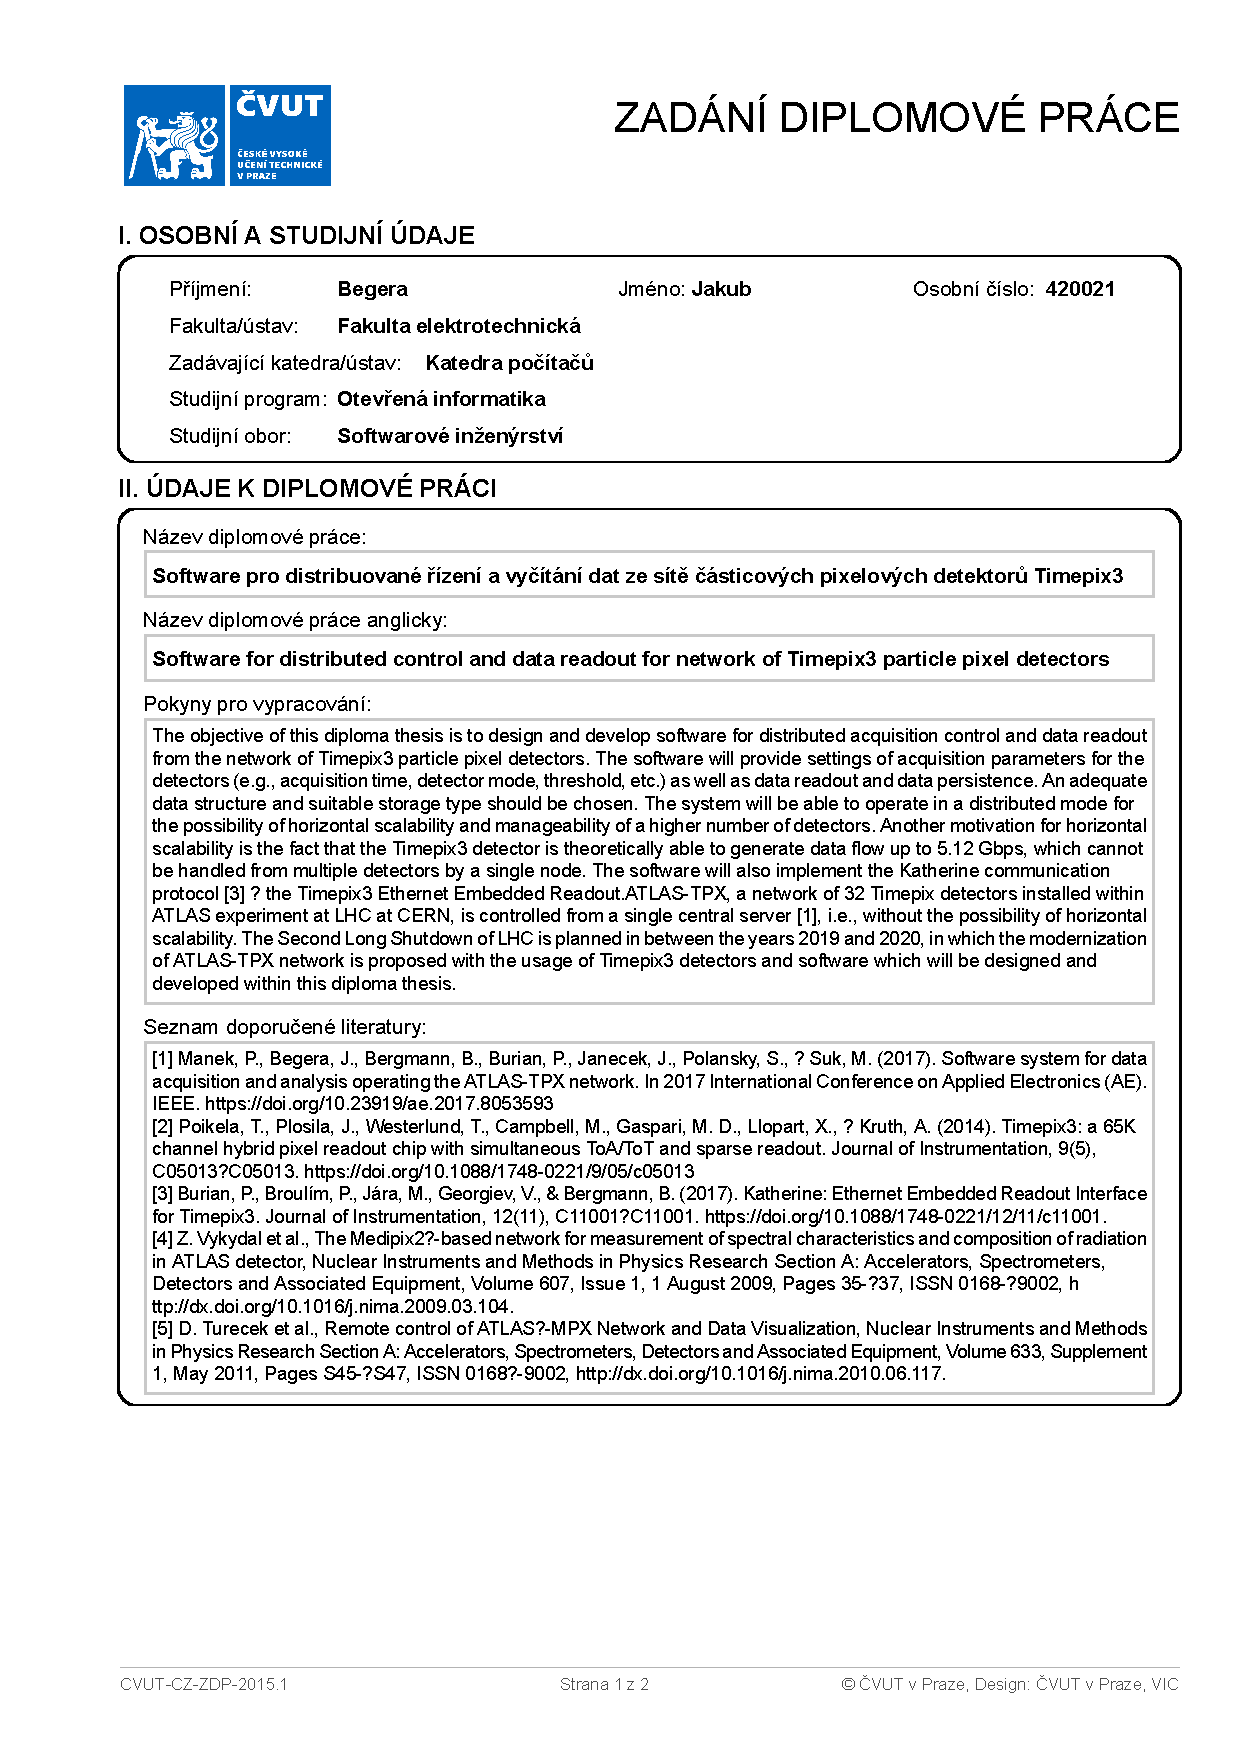
\includepdf[pages=1]{zadani.pdf}
	\newpage

	%%%%%%%%%%%%%%%%%%%%%%%%%%%    
	% Poděkovani / Acknowledgements 
	\acknowledgements
	\noindent
	\todo


	%%%%%%%%%%%%%%%%%%%%%%%%%%%   
	% Prohlášení / Declaration 

	\declaration{V~Praze dne 27.\,5.\,2016}


	%%%%%%%%%%%%%%%%%%%%%%%%%%%%    
	% Abstrakt / Abstract 
 
	\abstractpage

	\todo abstrakt anglicky

	
	\vglue60mm
	\noindent{\Huge \textbf{Abstrakt}}
	\vskip 2.75\baselineskip

	\todo abstrakt česky


	%%%%%%%%%%%%%%%%%%%%%%%%%%    
	% obsahy a~seznamy
	\tableofcontents		% Obsah
	\listoffigures			% Seznam obrázků
	\listoftables			% Seznam tabulek
	\listofcodes			% Seznam zdrojových kódů	

	%%%%%%%%%%%%%%%%%%%%%%%%%% 
	% začátek textu  
	\mainbodystarts

\addbibresource{reference.bib}

\chapter{Introduction}\label{chap01}
Test

\bibliographystyle{csplainnat}

{
%JZ: 11.12.2008 Kdo chce mit v~techto ukazkovych odkazech take odkaz na CSTeX:
\def\CS{$\cal C\kern-0.1667em\lower.5ex\hbox{$\cal S$}\kern-0.075em $}
\bibliography{reference}
}


%%%%%%%%%%%%%%%%%%%%%%%%%% 
% Přílohy
\appendix	

\printnomenclature
\label{apx:zkratky}

\chapter{Obsah přiloženého CD}\label{chap:app:cd}

\definecolor{fblue}{RGB}{92,144,192}
\definecolor{fgreen}{RGB}{34,162,70}

\def\Size{4pt}
\newcommand\myfolder[2][fblue]{%
\begin{tikzpicture}[overlay]
%\begin{scope}[xshift=20pt]
%\tikzset{
\filldraw[draw=folderborder,top color=folderbg!50,bottom color=folderbg]
      (-1.05*\Size,0.2\Size+5pt) rectangle ++(.75*\Size,-0.2\Size-5pt);  
    \filldraw[draw=folderborder,top color=folderbg!50,bottom color=folderbg]
      (-1.15*\Size,-\Size) rectangle (1.15*\Size,\Size);
%\end{scope}  
\end{tikzpicture}%
\makebox[2cm]{\raisebox{-3pt}{{\ttfamily#2}}}%
%}
}


\begin{figure}[th!]
\begin{center}
\begin{forest}
  for tree={
    font=\ttfamily,
    grow'=0,
    child anchor=west,
    parent anchor=south,
    anchor=west,
    calign=first,
    inner xsep=7pt,
    edge path={
      \noexpand\path [draw, \forestoption{edge}]
      (!u.south west) +(7.5pt,0) |- (.child anchor) \forestoption{edge label};
    },
    before typesetting nodes={
      if n=1
        {insert before={[,phantom]}}
        {}
    },
    fit=band,
    before computing xy={l=15pt},
  }  
[CD/
	[pixnet/
		[commons/ - modul se společnými závislosti]
		[detector\_communication\_intf/ - modul s komunikačním interface]
		[detector\_communication\_katherine/ - komunikační modul Katherine]
		[detector\_data\_persistence\_intf/ - modul s datovým interface]
		[handler/ - modul s handlerem]
		[katherine\_commons/ - společné závislosti Katherine modulů]
		[katherine\_emulator/ - emulátor Katherine]
		[katherine\_persistence\_file/ - datový modul Katherine]
		[master/ - modul s backendovou aplikací mastera]
	]
	[pixnet\_frontend/ - webová single-page aplikace]
	[text/
		[src/ - adresář se zdrojovými soubory tohoto dokumentu]
		[master-thesis-jakub-begera-2019.pdf - tato práce ve formátu PDF]
		[abstract\_cz.txt - abstrakt česky]
		[abstract\_en.txt - abstrakt anglicky]
	]
	[detector\_model.json - přehled příkazů komunikačního modulu Katherine]
]
\end{forest}
\end{center}
\caption{Obsah přiloženého CD}
\label{fig:attached-cd}
\end{figure}

\end{document}
